\documentclass[journal,12pt,twocolumn]{article}\usepackage[margin=1.25 in]{geometry}
\usepackage{amsmath, amssymb}
\usepackage{multicol}
\usepackage{graphicx}

\addtolength{\topmargin}{-.4 in}

\title{\LARGE{\textbf{Assignment-1}\\(ICSE 10, 2019)}}
\author{J Sai Sri Hari Vamshi\\ (AI21BTECH11014)}
\date{}

\begin{document}
\maketitle

\begin{center}
    \textbf{\large Problem 4(a):}
\end{center}
\begin{flushleft}
The following numbers, $K + 3, K + 2, 3K - 7$ and $2K - 3$ are in proportion. Find $K$.\\[2\baselineskip]
\end{flushleft}
\begin{center}
    \textbf{\large Solution:}
\end{center}

\noindent Given numbers,

\begin{align*}
a_1 & = K + 3\\
a_2 & = K + 2\\
a_3 & = 3K - 7\\
a_4 & = 2K - 3\\
\end{align*}

\noindent For the Proportionality of the numbers, they must satisfy,

\[ \frac{a_1}{a_2} = \frac{a_3}{a_4} \]

\noindent So we get,

\[ \frac{K + 3}{K + 2} = \frac{3K - 7}{2K - 3} \]

\noindent By cross multiplication,

\begin{align*}
    (K + 3)(2K - 3) & = (3K - 7)(K + 2)\\
    2K^2 + 3K - 9 & = 3K^2 - K - 14\\
    K^2 - 4K - 5 & = 0\\
    K^2 - 5K + K - 5 & = 0\\
    (K - 5)(K + 1) & = 0\\
\end{align*}

\noindent From above $K$ will either be $5$ or $-1$.\\

\noindent See Figure
	  \ref{Figure_1_py.png}.
  \begin{figure}
	  \centering 
	  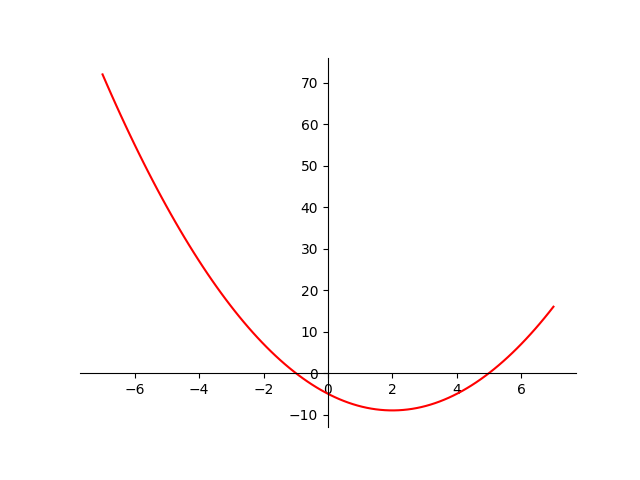
\includegraphics[width=\columnwidth]{Figure_1_py.png}
	  \caption{The Polynomial graph}
	  \label{Figure_1_py.png}
	  \end{figure}

\end{document}